% scRareRefine Chinese draft typeset from the supplied Springer Nature template.
% The template's original Math and Physical Sciences numbered-reference class is retained.
\documentclass[pdflatex,sn-mathphys-num]{sn-jnl}

\usepackage[UTF8,scheme=plain]{ctex}
\usepackage{graphicx}
\usepackage{multirow}
\usepackage{amsmath,amssymb,amsfonts}
\usepackage{amsthm}
\usepackage{mathrsfs}
\usepackage[title]{appendix}
\usepackage{xcolor}
\usepackage{textcomp}
\usepackage{manyfoot}
\usepackage{booktabs}
\usepackage{algorithm}
\usepackage{algorithmicx}
\usepackage{algpseudocode}
\usepackage{listings}

%% The following theorem styles are retained from template.tex.
\theoremstyle{thmstyleone}%
\newtheorem{theorem}{Theorem}%
\newtheorem{proposition}[theorem]{Proposition}%
\theoremstyle{thmstyletwo}%
\newtheorem{example}{Example}%
\newtheorem{remark}{Remark}%
\theoremstyle{thmstylethree}%
\newtheorem{definition}{Definition}%

\graphicspath{{./}{figures/}}
\newcommand{\method}{scRareRefine}
\newcommand{\rare}{r}
\newcommand{\rts}{\texttt{rare\_train\_size}}
\newcommand{\train}{\mathrm{train}}
\newcommand{\valsplit}{\mathrm{val}}
\newcommand{\testsplit}{\mathrm{test}}
\DeclareMathOperator*{\argmax}{arg\,max}

\raggedbottom

\begin{document}

% User-requested exception: author--year citations in the text, numbered entries in References.
\setcitestyle{authoryear,round,semicolon}

\title[验证集校准的稀有细胞拯救]{稀有标签匮乏条件下低频目标细胞的验证集校准事后拯救}

\author*[1]{\fnm{Jiahao} \sur{Zhou}}\email{jhzhou0704@163.com}
\affil*[1]{\orgdiv{数学与系统科学学院}, \orgname{新疆大学},
  \orgaddress{\city{乌鲁木齐}, \state{新疆}, \country{中国}}}

\abstract{当稀有类别仅有少量标注样本时，半监督单细胞注释模型可能漏检一个已知的低频目标细胞类型。本文提出\method，一种用于冻结 scANVI 骨干模型的事后细化模块。该方法结合训练集估计的潜在空间原型、训练集导出的可分性门控，以及验证集驱动的必要性守门、候选秩选择和 conformal 分数阈值校准，并面向预先指定的目标类别，而非从头发现稀有细胞群。在 8 个涵盖人和小鼠的单细胞 RNA 测序数据集中，仅保留训练集中 1\%、5\% 或 10\% 的稀有细胞标签后，有标签稀有细胞仅占全部训练细胞的 0.0206\%--0.3526\%。在该区域，\method 的平均稀有细胞 F1 为 0.801，scANVI 和 kNN 分别为 0.646 和 0.665；在按三个随机种子聚合得到的 24 个数据集--稀缺预算组合中，\method 在 23 个组合上取得最高或并列最高的平均稀有细胞 F1。在所有评估运行中，最终预测的最大观测总体稀有类假调用率为 0.009878，低于 0.01 的预设参考预算。结果表明，验证集校准的保守事后拯救可以在恢复稀有细胞召回率的同时经验性抑制假阳性扩张。}

\keywords{单细胞 RNA 测序, 稀有细胞注释, 半监督学习, conformal 校准, 事后细化}

\maketitle

\section{引言}

单细胞 RNA 测序使复杂组织的细胞分辨率分析成为常规手段，但最具生物学意义的细胞类型往往并非数量最多的类型。稀有免疫亚群、内分泌亚型、组织驻留基质细胞和谱系中间状态可能仅占数据集的几个百分点，其标签也最为脆弱。小型参考面板只能提供少量阳性样本，按批次留出的评估可能使目标类别处于不同技术环境，而半监督分类器可能将代表不足的类别合并到邻近多数类别中。

由此形成一种实际的细胞类型注释失效模式，即模型可获得尚可的总体准确率，却系统性丢失研究关注的细胞类型。问题不仅在于类别在完整数据集中的丰度。对于监督或半监督模型，更直接的量是训练细胞中目标稀有类别有标签样本所占比例。本文所有正式目标类别在数据集层面的丰度均低于 5\%，而在训练集下采样稀有标签后，主要稀缺标签设置中的有标签稀有细胞仅占全部训练细胞的 0.0206\%--0.3526\%。

\paragraph{相关工作。}
现有注释方法从不同方向处理这一问题。scANVI 从有标签和无标签细胞中学习半监督潜在表示与分类器\citep{lopez2018scvi,xu2021scanvi}。CellTypist、TOSICA 及相关监督系统利用标志基因信息或 Transformer 模型实现可扩展注释\citep{dominguez2022celltypist,chen2023tosica}。scBalance 和 scCAD 等重平衡或稀有细胞检测方法旨在缓解类别不平衡或发现异常细胞群\citep{cheng2023scbalance,xu2024sccad}。ProtoCloud 等原型方法使用参考标签的几何摘要，HiCat 则结合监督参考信息与转导聚类\citep{guo2026protocloud,bi2025hicat}。这些方法具有重要价值，但没有直接回答一个特定部署问题，即当半监督分类器漏检已知低频目标类别时，能否在约束稀有细胞假调用的同时选择性恢复可能的假阴性。

\method 针对上述场景设计。它不是从头发现稀有细胞的方法，也不改变 scANVI 的训练目标，而是在 scANVI 之后应用的归纳式事后模块。该模块由有标签训练细胞构建潜在空间原型，根据目标稀有原型相对于其他类别原型的接近程度对候选细胞评分，并使用验证细胞决定是否需要拯救以及规则应具有多大宽容度。最终重标记阈值由验证集非稀有细胞以 $\alpha=0.01$ 为目标进行校准。若目标类别在几何上不可分、基线已恢复验证集稀有细胞，或没有候选秩满足验证集安全标准，方法将弃权并返回基线预测。图~\ref{fig:overview} 概述了该流程。

本文在 8 个数据集上比较\method 与 8 个基线或替代方法，数据覆盖人和小鼠、多种组织、3 个随机种子以及 4 个稀有标签预算。基准包含 6 个人类数据集和 2 个小鼠 Tabula Muris Senis 10x 附加数据集，在保持各数据集内部训练、验证和测试评估的同时扩展了组织与物种覆盖面。本文检验的主要主张是，\method 能够在以 $\alpha=0.01$ 为校准目标的条件下恢复标签匮乏时的稀有细胞注释，并在缺乏拯救依据时弃权。

\paragraph{主要贡献。}
本文提出一个面向已知低频目标类别的全归纳式事后拯救模块。该模块采用训练集导出的可分性安全网，以及三个验证集驱动的步骤：必要性守门、候选秩选择和以 $\alpha=0.01$ 为目标的分数阈值校准。本文区分数据集层面的目标丰度 $\pi_r=N_r/N<5\%$ 与训练时的有效有标签稀有比例 $\lambda_r=L_{r,\mathrm{train}}/N_{\mathrm{train}}$。在 8 个数据集、9 种方法、4 个标签预算和 3 个随机种子的比较中，\method 在稀缺标签区域取得最高平均稀有细胞 F1，并在按三个随机种子聚合得到的 24 个数据集--稀缺预算组合中的 23 个上取得最高或并列最高的平均稀有细胞 F1。在所有评估运行中，最终预测的最大观测总体稀有类假调用率为 0.009878，低于 1\% 的预设参考预算。本文同时明确方法仅用于已知目标类别的事后拯救，并讨论无操作情形、几何纠缠以及尚未进行直接人到小鼠迁移评估等限制。

\begin{figure}[t]
\centering
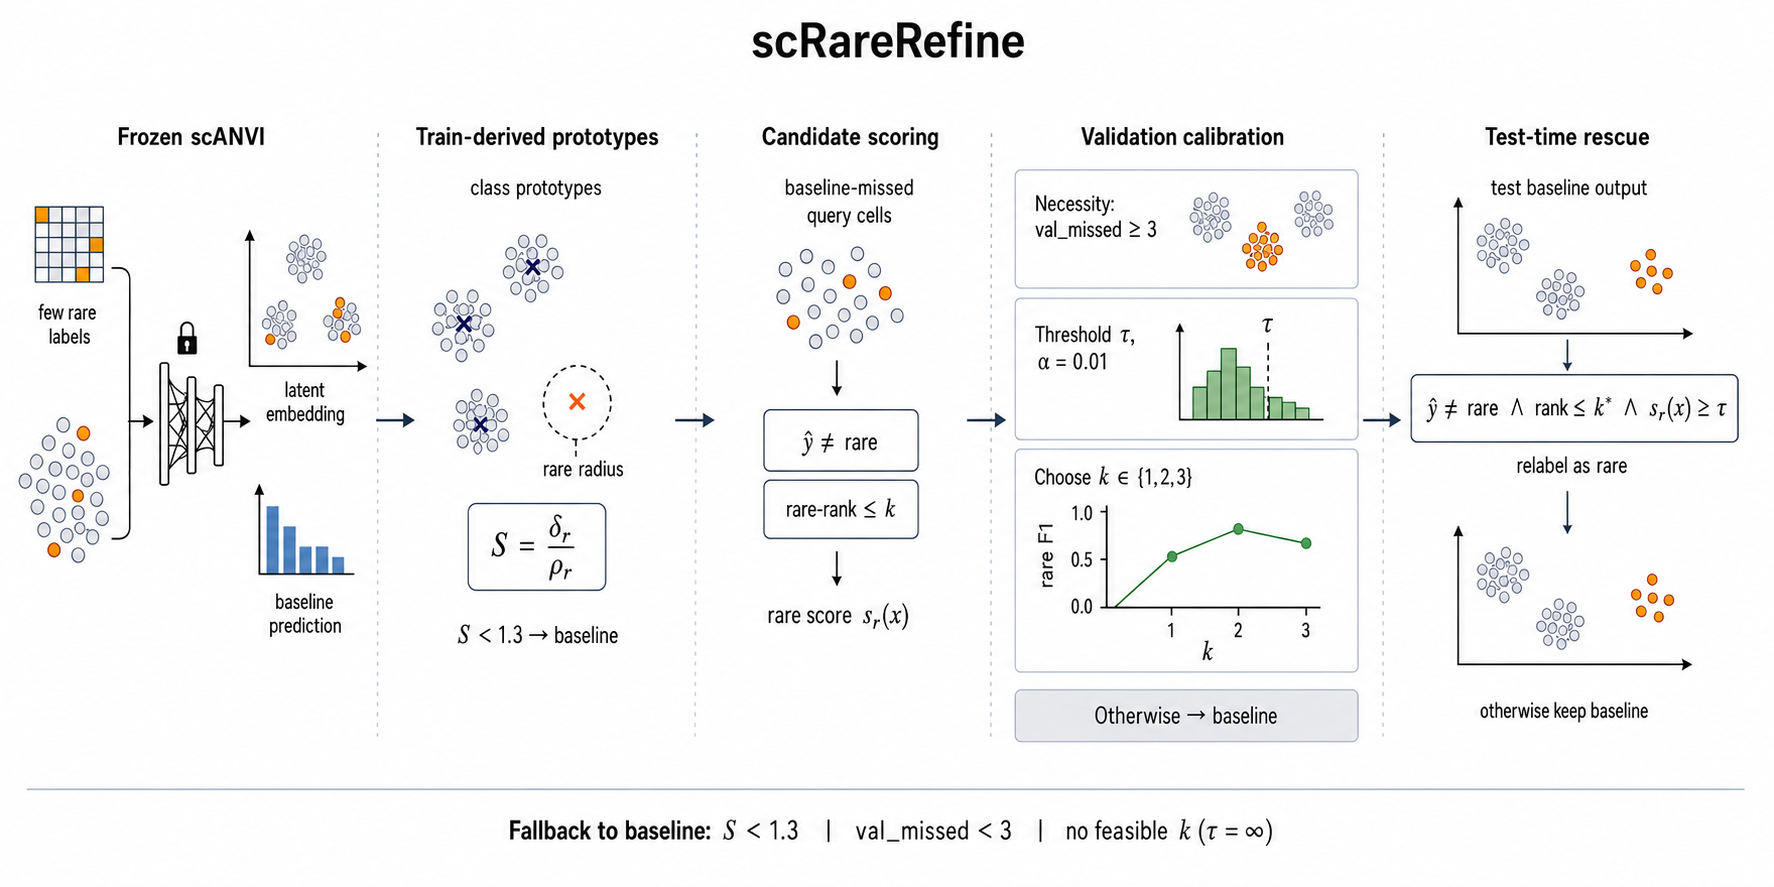
\includegraphics[width=\linewidth]{fig1_overview.png}
\caption{\method 工作流程。scANVI 提供潜在嵌入和初始预测；\method 拟合仅基于训练集的原型，应用训练集可分性门控，由验证集完成必要性守门、候选秩选择与分数阈值校准，最后在留出测试细胞上评估拯救结果。}
\label{fig:overview}
\end{figure}

\section{系统与方法}

\subsection{问题设置}

设单细胞数据集包含基因表达矩阵 $X$、部分细胞的细胞类型标签 $y$，以及预先指定的目标稀有类别 $\rare$。目标类别由数据集配置给出，而非根据频率阈值自动推断。完整标签数据仅用于定义评估目标，随后构造归纳式训练集、验证集和测试集。模型拟合、原型估计、候选秩选择和阈值校准仅使用训练与验证信息，测试标签只用于最终评估。

本文区分两种稀有性。第一种是数据集层面的目标丰度
\[
  \pi_\rare=N_\rare/N,
\]
其中 $N_\rare$ 为配置的目标稀有类别细胞数，$N$ 为数据集规模。排除探索性 \texttt{tabula\_lung\_stroma} 数据集后，正式基准中所有目标类别均满足 $\pi_\rare<5\%$。第二种是训练集的稀有标签可用性
\[
  \lambda_\rare=L_{\rare,\mathrm{train}}/N_{\mathrm{train}},
\]
其中 $L_{\rare,\mathrm{train}}$ 是下采样后保留的有标签稀有训练细胞数，$N_{\mathrm{train}}$ 是训练细胞总数。标签预算 \rts{} $=0.01,0.05,0.10$ 分别保留约 1\%、5\% 或 10\% 的训练稀有标签，在条件允许时至少保留 5 个；\rts{} $=$ \texttt{all} 保留全部训练稀有标签。在 8 个正式数据集和 3 个随机种子中，稀缺标签设置对应 $\lambda_\rare=0.0206\%$--$0.3526\%$。表~\ref{tab:target-abundance} 和表~\ref{tab:labeled-ratio} 分别报告这两个层面的稀有性。

\begin{table}[t]
\centering
\caption{预先指定目标类别的数据集层面丰度。所有正式基准目标均满足 $\pi_r=N_r/N<5\%$。}
\label{tab:target-abundance}
\scriptsize
\begin{tabular}{p{0.28\linewidth}p{0.34\linewidth}rrr}
\toprule
数据集 & 目标类别 & $N$ & $N_r$ & $\pi_r$（\%）\\
\midrule
\texttt{immune\_dc} & ASDC & 23287 & 522 & 2.24 \\
\texttt{mouse\_lung\_tms\_10x} & vein endothelial cell & 24536 & 320 & 1.30 \\
\texttt{mouse\_pancreas\_tms\_10x} & pancreatic D cell & 6201 & 272 & 4.39 \\
\texttt{pancreas\_baron} & gamma & 8569 & 255 & 2.98 \\
\texttt{pancreas\_integrated} & endothelial & 10963 & 273 & 2.49 \\
\texttt{tabula\_lung\_endo} & endothelial cell of lymphatic vessel & 10132 & 307 & 3.03 \\
\texttt{tabula\_sapiens\_stomach} & mast cell & 33064 & 968 & 2.93 \\
\texttt{tabula\_small\_intestine} & intestinal tuft cell & 40350 & 435 & 1.08 \\
\bottomrule
\end{tabular}
\end{table}

\begin{table}[t]
\centering
\caption{训练集中的有效有标签稀有比例 $\lambda_r=L_{r,\mathrm{train}}/N_{\mathrm{train}}$。各列表示保留为有标签样本的训练稀有细胞比例，表中数值为其占全部训练细胞的百分比。}
\label{tab:labeled-ratio}
\scriptsize
\begin{tabular}{lrrrr}
\toprule
数据集 & 1\% 有标签 & 5\% 有标签 & 10\% 有标签 & 全部有标签\\
\midrule
\texttt{immune\_dc} & 0.0443 & 0.1151 & 0.2391 & 2.4533 \\
\texttt{mouse\_lung\_tms\_10x} & 0.0232 & 0.0463 & 0.0973 & 0.9868 \\
\texttt{mouse\_pancreas\_tms\_10x} & 0.1037 & 0.1659 & 0.3526 & 3.6092 \\
\texttt{pancreas\_baron} & 0.0902 & 0.0902 & 0.1804 & 1.9127 \\
\texttt{pancreas\_integrated} & 0.0630 & 0.1512 & 0.3024 & 3.0620 \\
\texttt{tabula\_lung\_endo} & 0.0670 & 0.1340 & 0.2680 & 2.7867 \\
\texttt{tabula\_sapiens\_stomach} & 0.0350 & 0.0350 & 0.0350 & 0.3642 \\
\texttt{tabula\_small\_intestine} & 0.0206 & 0.0618 & 0.1277 & 1.2973 \\
\bottomrule
\end{tabular}
\end{table}

\subsection{数据划分与标签掩蔽}

主要实验采用按批次留出划分。若元数据支持该设计，则按批次将细胞划分为训练、验证和测试集，其他情形由预处理流程中的回退逻辑处理。由于各批次规模不同，实际划分比例不必与名义比例完全一致，但划分在模型拟合前固定，并记录于运行清单。该设计评估稀有细胞恢复规则能否跨留出的实验批次迁移，而非仅在随机抽样细胞之间迁移。

训练集内部按照所选标签预算对稀有类别标签下采样。非稀有有标签细胞保持可用，而标签被掩蔽的稀有细胞在半监督训练中视为无标签。验证与测试标签不作下采样。验证标签仅用于方法选择与校准，测试标签仅用于最终指标。对于比例预算 $b\in\{0.01,0.05,0.10\}$，训练集中保留的稀有标签数为
\[
L_{\rare,\train}(b)=\min\{N_{\rare,\train},\max(5,\lfloor bN_{\rare,\train}\rfloor)\},
\]
这与实现中对稀缺稀有类别采用的 5 细胞下限一致。对于 \rts{} $=$ \texttt{all}，有 $L_{\rare,\train}=N_{\rare,\train}$。

\subsection{scANVI 骨干与原型评分}

骨干模型为 scANVI，通过 scvi-tools 在流程内选择的高变基因上训练。模型首先使用 scVI 学习潜在表示，随后利用有标签和无标签训练细胞拟合半监督 scANVI 分类器。流程为每个划分导出预测标签、类别概率和潜在嵌入。\method 及适用的比较脚本共享这些嵌入，并通过清单检查避免在不兼容配置、划分或数据集之间误用缓存。

\method 使用有标签训练细胞在 scANVI 潜在空间中构建类别原型。令 $\mathcal{I}_c=\{i:i\in\train,y_i=c,i\text{ 有标签}\}$，$z_i\in\mathbb{R}^d$ 为导出的潜在嵌入，则
\[
\mu_c=\frac{1}{|\mathcal{I}_c|}\sum_{i\in\mathcal{I}_c}z_i,\qquad
\rho_c=\max\left\{\operatorname{median}_{i\in\mathcal{I}_c}\|z_i-\mu_c\|_2,10^{-6}\right\}.
\]
若可用有标签样本少于 3 个，则令 $\rho_c=1$。训练集可分性门控定义为
\[
\eta_\rare=\frac{\min_{c\ne\rare}\|\mu_\rare-\mu_c\|_2}
{|\mathcal{I}_\rare|^{-1}\sum_{i\in\mathcal{I}_\rare}\|z_i-\mu_\rare\|_2},
\]
当 $\eta_\rare<1.3$ 时方法弃权。

稀有成员分数由归一化原型距离计算，使相对于竞争原型更接近目标稀有原型的细胞获得更高分数：
\[
s_i=\frac{\exp\{-\|z_i-\mu_\rare\|_2/\rho_\rare\}}
{\sum_c\exp\{-\|z_i-\mu_c\|_2/\rho_c\}}.
\]
同时计算稀有原型的未归一化欧氏距离秩
\[
\operatorname{rank}_i(\rare)=1+\sum_{c\ne\rare}\mathbb{I}\{\|z_i-\mu_c\|_2<\|z_i-\mu_\rare\|_2\}.
\]
仅当 scANVI 预测 $\hat y_i$ 不是目标稀有类别且
\[
q_i(k)=\mathbb{I}\{\hat y_i\ne\rare,\operatorname{rank}_i(\rare)\le k\}=1
\]
时，细胞才被视为拯救候选，其中 $k$ 由验证数据从 $\{1,2,3\}$ 中选择。

\subsection{训练集可分性门控与验证集校准}

\method 在重标记测试细胞前使用一个训练集导出的可分性安全网，以及三个验证集驱动的步骤：必要性守门、候选秩选择和分数阈值校准。训练集可分性门控比较目标稀有原型与最近非稀有原型的距离及稀有类别内半径；当 $\eta_\rare<1.3$ 时，方法弃权并返回基线预测。该常数预先固定，不针对单个数据集调节。

必要性守门统计验证集中被 scANVI 基线漏检的真实稀有细胞数 $M_{\rare,\valsplit}$。当 $M_{\rare,\valsplit}<3$ 时，\method 弃权。该规则既覆盖验证集稀有召回率达到 1 的无拯救必要情形，也避免仅凭 1--2 个漏检样本选择候选秩。

随后由验证集真实非稀有细胞校准稀有分数阈值。令 $S_0=\{s_i:i\in\valsplit,y_i\ne\rare\}$，排序后为 $s_{(1)}\le\cdots\le s_{(m)}$。以 $\alpha=0.01$ 为校准目标的有限样本高分位阈值为\citep{vovk2005algorithmic,angelopoulos2023conformal}
\[
\tau_\alpha=
\begin{cases}
s_{(\ell)},&\ell=\lceil(1-\alpha)(m+1)\rceil\le m,\\
+\infty,&\ell>m.
\end{cases}
\]

固定 $\tau_\alpha$ 后，方法对每个 $k\in\{1,2,3\}$ 计算验证集稀有 F1 和总体稀有类假调用率。设验证集真实非稀有细胞数为 $n$，其中被最终规则错误预测为稀有类的细胞数为 $x_k$，且 $\widehat p_k=x_k/n$。代码使用 $z=1.96$，并计算双侧 95\% Wilson score 区间的上端点
\[
U_{\mathrm{Wilson}}(k)=
\frac{\widehat p_k+\frac{z^2}{2n}+z\sqrt{\frac{\widehat p_k(1-\widehat p_k)}{n}+\frac{z^2}{4n^2}}}
{1+\frac{z^2}{n}},\qquad z=1.96.
\]
仅当 $U_{\mathrm{Wilson}}(k)\le\alpha$ 时，候选秩才可行。在可行集合中选择验证集稀有 F1 最大的 $k$，平局时选择较小的秩：
\[
k^\star=\argmax_{k\in\{1,2,3\}:\,U_{\mathrm{Wilson}}(k)\le\alpha}
\mathrm{F1}_{\rare,\valsplit}(k).
\]
若不存在可行候选秩，流程弃权并返回基线预测。测试时的预测为
\[
\tilde y_i=
\begin{cases}
\rare,&\hat y_i\ne\rare,\ \operatorname{rank}_i(\rare)\le k^\star,\ s_i\ge\tau_\alpha,\\
\hat y_i,&\text{其他情况。}
\end{cases}
\]

\begin{algorithm}[H]
\caption{面向一个预先配置目标类别的 \method 事后拯救流程}
\label{alg:scrarerefine}
\small
\begin{algorithmic}[1]
\Require 冻结 scANVI 在训练、验证和测试集上的潜在嵌入与预测；目标类别 $\rare$；校准目标 $\alpha=0.01$
\State 仅用有标签训练细胞拟合各类别原型 $\mu_c$ 与半径 $\rho_c$
\State 由训练原型计算目标类别可分性 $\eta_\rare$
\If{$\eta_\rare<1.3$}
  \State \Return scANVI 基线测试预测
\EndIf
\State 统计验证集中被基线漏检的稀有细胞数 $M_{\rare,\valsplit}$
\If{$M_{\rare,\valsplit}<3$}
  \State \Return scANVI 基线测试预测
\EndIf
\State 计算验证和测试细胞的稀有原型成员分数及原型距离秩
\State 用验证集真实非稀有细胞的分数校准阈值 $\tau_\alpha$
\For{$k\in\{1,2,3\}$}
  \State 用固定的 $\tau_\alpha$ 和 $k$ 计算验证集稀有 F1
  \State 以 $z=1.96$ 计算验证集总体稀有类假调用率的双侧 95\% Wilson 区间上端点 $U_{\mathrm{Wilson}}(k)$
\EndFor
\State 保留满足 $U_{\mathrm{Wilson}}(k)\le\alpha$ 的候选秩
\If{可行候选集合为空}
  \State \Return scANVI 基线测试预测
\EndIf
\State 选择验证集稀有 F1 最大的 $k^\star$；平局时选择较小的秩
\For{每个测试细胞 $i$}
  \If{$\hat y_i\ne\rare$，且 $\operatorname{rank}_i(\rare)\le k^\star$，且 $s_i\ge\tau_\alpha$}
    \State 将该细胞重标记为 $\rare$
  \EndIf
\EndFor
\State \Return 细化后的测试预测
\end{algorithmic}
\end{algorithm}

\subsection{数据集、比较方法与指标}

正式基准包含 8 个数据集。6 个人类数据集覆盖免疫、胰腺、肺、胃和小肠，另加入 2 个小鼠 Tabula Muris Senis 10x 数据集以扩展物种与组织覆盖。目标稀有类别在数据集配置文件中预先固定，并非依据模型性能事后选择。人类数据来源包括 AIFI Human Immune Health Atlas、Baron 胰腺研究、scIB 胰腺整合基准和 Tabula Sapiens；小鼠数据来自 Tabula Muris Senis\citep{gong2025immuneatlas,baron2016pancreas,luecken2022scib,tabulasapiens2022,tabulamurissenis2020}。登录号、稳定下载页和项目特定子集规则见补充表 S5。

本文比较\method、scANVI、共享潜在表示上的 kNN、CellTypist、scBalance、ProtoCloud、HiCat、scCAD 和 TOSICA。适用时，所有方法均在相同数据划分、随机种子和稀有标签预算上评估。完整结果表包含 864 个成功的方法级评估记录，覆盖 $8\times4\times3=96$ 个数据集--标签预算--随机种子单元，每个单元评估 9 种方法。相同单元内的方法共享预先固定的数据划分；kNN 与 \method 还共享 scANVI 潜在表示，因此这些记录不应解释为 864 次相互独立的端到端训练。HiCat 作为转导式参考单独标注，其结果不与完全归纳式方法作等价解释。

主要指标为独立测试集上的稀有类别 F1，同时报告稀有类别精确率和召回率。跨方法安全指标为真实非稀有细胞中的总体稀有假调用率 \texttt{rare\_fp\_rate}，其中包含基线错误及细化引入的错误。对于\method，另报告 \texttt{rescue\_ffr}，即事后模块新重标记细胞造成的增量假拯救率，并使用相同的真实非稀有分母。稀缺标签区域定义为 \rts{} $\in\{0.01,0.05,0.10\}$。指标定义为
\[
\mathrm{Precision}_\rare=\frac{\mathrm{TP}_\rare}{\mathrm{TP}_\rare+\mathrm{FP}_\rare},\quad
\mathrm{Recall}_\rare=\frac{\mathrm{TP}_\rare}{\mathrm{TP}_\rare+\mathrm{FN}_\rare},\quad
\mathrm{F1}_\rare=\frac{2\,\mathrm{Precision}_\rare\,\mathrm{Recall}_\rare}{\mathrm{Precision}_\rare+\mathrm{Recall}_\rare}.
\]
总体稀有假调用率为
\[
\mathrm{FRCR}_\rare=\frac{\mathrm{FP}_\rare}{|\{i\in\testsplit:y_i\ne\rare\}|},
\]
其中 $\mathrm{FP}_\rare$ 包含基线已有错误和事后拯救新增错误。增量假拯救率只统计由事后模块新增的错误重标记：
\[
\mathrm{rescue\_ffr}=
\frac{|\{i\in\testsplit:y_i\ne\rare,\ \hat y_i\ne\rare,\ \tilde y_i=\rare\}|}
{|\{i\in\testsplit:y_i\ne\rare\}|}.
\]
全文将前者称为总体稀有类假调用率（total rare-class false-call rate, FRCR），将后者称为增量假拯救率（incremental rescue FFR）。二者均与预先指定的 $\alpha=0.01$ 参考预算作经验比较。在校准集与测试集可交换的条件下，conformal 分数阈值具有通常的有限样本解释。然而，主要基准留出完整批次，并额外在验证集上选择候选秩。因此，本文报告分布偏移下的经验假调用行为，而不声称完整流程具有无条件 conformal 保证。

\section{结果}

\subsection{稀有标签匮乏比目标类别低丰度更为严重}

所有正式目标类别在各自数据集中均为低频类别，完整数据集丰度低于 5\%。然而，标签匮乏实验的难度取决于训练过程可获得的有标签稀有细胞数。在最严格的设置中，分类器面对数千个非稀有训练细胞时只能看到少量稀有标签。例如，在 \texttt{immune\_dc} 的 \rts{} $=0.01$ 设置中，训练集包含 277 个稀有细胞和 11014 个非稀有细胞，但仅有 5 个稀有细胞保留标签，因此 $\lambda_\rare=5/(277+11014)=0.0443\%$。

这一表述澄清了评估目标。本任务不是发现低于固定频率阈值的任意细胞簇，而是在有标签阳性样本稀少到半监督分类器可能从预测中抹去该类别时，保留并恢复一个已知低频类别。图~\ref{fig:scarcity-recovery} 同时展示有效训练标签匮乏程度及相应的 F1 和召回恢复曲线。

\begin{figure}[t]
\centering
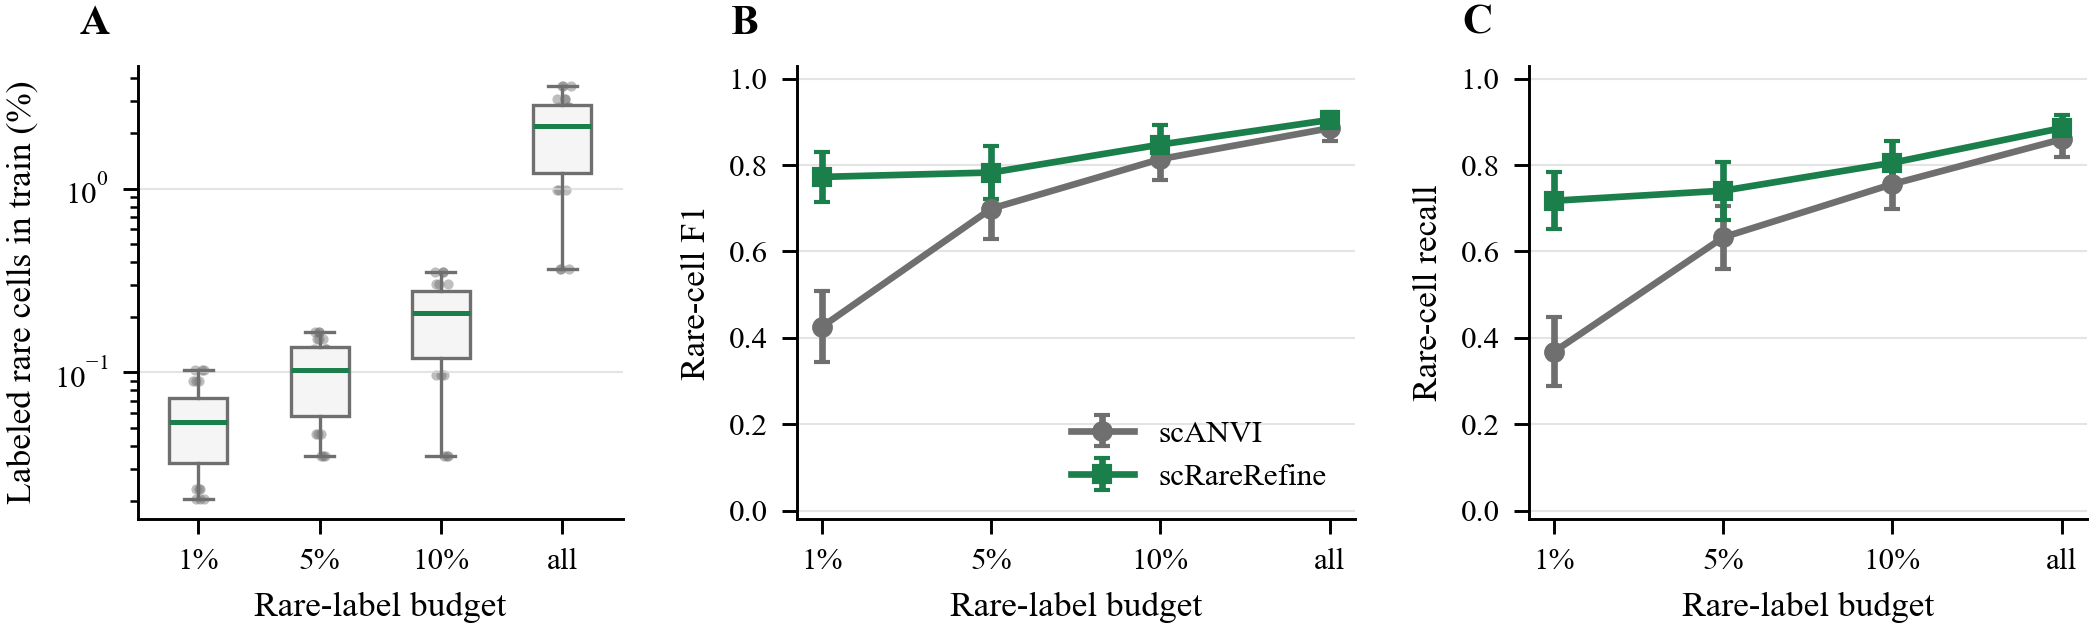
\includegraphics[width=\linewidth]{fig2_label_scarcity_recovery.png}
\caption{不同标签预算下的稀有标签匮乏与恢复。（A）有标签稀有细胞占全部训练细胞的百分比。（B、C）scANVI 与\method 在 8 个数据集和 3 个随机种子上的平均稀有细胞 F1 与召回率，误差条表示以运行作为单位计算的标准误。}
\label{fig:scarcity-recovery}
\end{figure}

\subsection{\method 在稀缺标签设置中提高稀有细胞 F1}

在稀缺标签区域，\method 获得所有方法中最高的平均稀有细胞 F1。对数据集、随机种子和稀缺标签预算取平均后，其稀有细胞 F1 为 0.8008，而 kNN 和 scANVI 分别为 0.6645 和 0.6463。提升主要来自召回恢复，\method 的平均稀有召回率为 0.7543，kNN 和 scANVI 分别为 0.5883 和 0.5855。

\begin{table}[t]
\centering
\caption{稀缺标签设置中的平均性能。平均和最大总体 FRCR 均基于最终预测；最大值取全部稀缺标签运行中的最大值。}
\label{tab:scarce}
\small
\begin{tabular}{lrrrr}
\toprule
方法 & 稀有 F1 & 召回率 & 平均总体 FRCR & 最大总体 FRCR\\
\midrule
\method & 0.8008 & 0.7543 & 0.0012 & 0.0098 \\
kNN & 0.6645 & 0.5883 & 0.0002 & 0.0035 \\
scANVI & 0.6463 & 0.5855 & 0.0003 & 0.0023 \\
scBalance & 0.5827 & 0.4967 & 0.0001 & 0.0021 \\
ProtoCloud & 0.5592 & 0.4776 & 0.0002 & 0.0018 \\
CellTypist & 0.5514 & 0.4688 & 0.0002 & 0.0012 \\
scCAD & 0.4726 & 0.6698 & 0.0246 & 0.0752 \\
TOSICA & 0.4345 & 0.3918 & 0.0030 & 0.0209 \\
HiCat & 0.1445 & 0.1193 & 0.0000 & 0.0002 \\
\bottomrule
\end{tabular}
\end{table}

按三个随机种子聚合后得到 24 个数据集--稀缺预算组合。\method 在其中 23 个组合上取得最高或并列最高的平均稀有细胞 F1。唯一未取得最佳的组合是 \texttt{tabula\_small\_intestine} 的 \rts{} $=0.10$，ProtoCloud 的稀有 F1 为 0.9848，\method 为 0.9823，差异为 0.0025。主要稀缺标签比较与安全性概况见图~\ref{fig:scarce-benchmark}。

\begin{figure}[t]
\centering
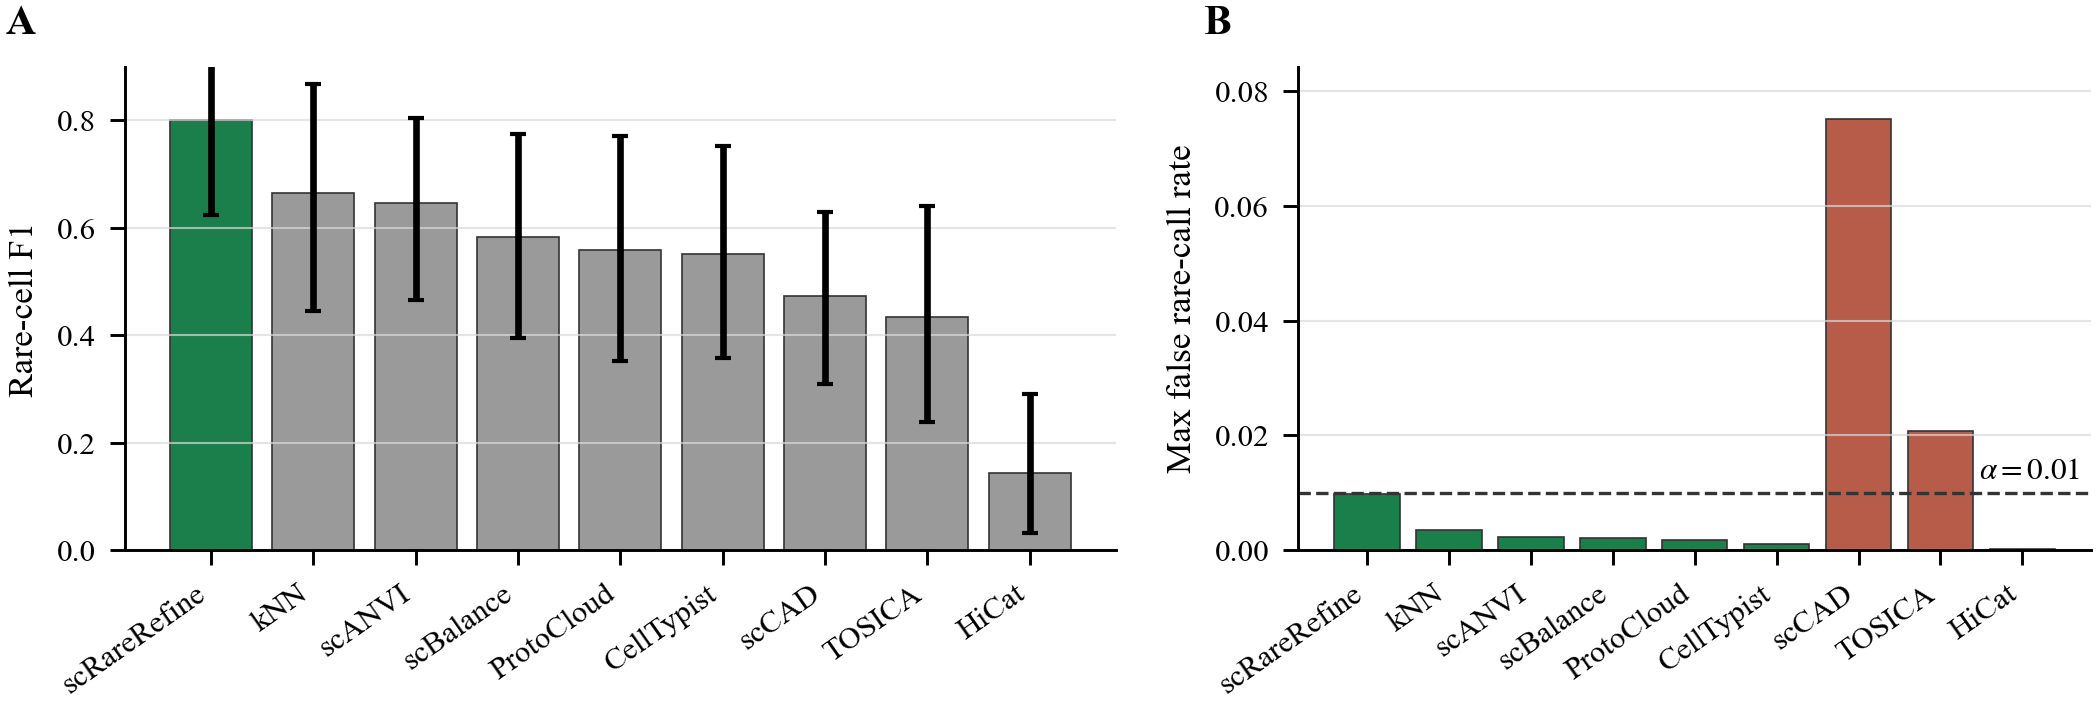
\includegraphics[width=\linewidth]{fig3_scarce_benchmark.png}
\caption{稀缺标签基准汇总。（A）按数据集等权计算的平均稀有细胞 F1，95\% 置信区间通过以数据集为簇重采样得到。（B）同一稀缺标签区域中的最大总体稀有假调用率，虚线表示预先指定的 $\alpha=0.01$ 参考预算。}
\label{fig:scarce-benchmark}
\end{figure}

\subsection{配对比较显示一致增益}

本文在稀缺标签区域按数据集、预算和随机种子匹配的单位中，将\method 与各方法比较。每个比较方法包含 72 个相关的匹配运行单位，胜、平、负计数用于描述这些运行，而统计推断将 8 个数据集作为独立单位。在每个数据集内，先对 3 个稀缺预算和 3 个随机种子的配对差异取平均，主要估计量为 8 个数据集效应的等权平均。相对于 scANVI，\method 在运行层面有 41 胜、30 平和 1 负；按数据集等权的平均 $\Delta$F1 为 $+0.1545$，数据集聚类 bootstrap 95\% 置信区间为 $[+0.0908,+0.2259]$。7 个平均效应非零的数据集均支持\method，另 1 个数据集的平均效应恰为零，双侧精确符号检验 $P=0.0156$。较多平局符合预期，因为当验证证据表明拯救不必要或不安全时，\method 会返回基线预测。图~\ref{fig:paired-delta} 汇总相对于全部比较方法的配对效应量。

\begin{table}[t]
\centering
\caption{稀缺标签区域的配对稀有 F1 比较。差异按数据集、稀有标签预算和随机种子配对。}
\label{tab:paired}
\small
\begin{tabular}{lrrrrr}
\toprule
比较方法 & 胜 & 平 & 负 & 平均 $\Delta$F1 & 95\% CI\\
\midrule
scANVI & 41 & 30 & 1 & +0.1545 & [+0.0908,+0.2259] \\
kNN & 59 & 8 & 5 & +0.1363 & [+0.0529,+0.2379] \\
CellTypist & 65 & 4 & 3 & +0.2494 & [+0.1411,+0.3493] \\
scBalance & 61 & 5 & 6 & +0.2181 & [+0.1249,+0.3150] \\
ProtoCloud & 62 & 6 & 4 & +0.2416 & [+0.1296,+0.3527] \\
HiCat & 66 & 5 & 1 & +0.6563 & [+0.5066,+0.7903] \\
scCAD & 66 & 5 & 1 & +0.3282 & [+0.2430,+0.4089] \\
TOSICA & 67 & 2 & 3 & +0.3663 & [+0.2237,+0.5003] \\
\bottomrule
\end{tabular}
\end{table}

\begin{figure}[t]
\centering
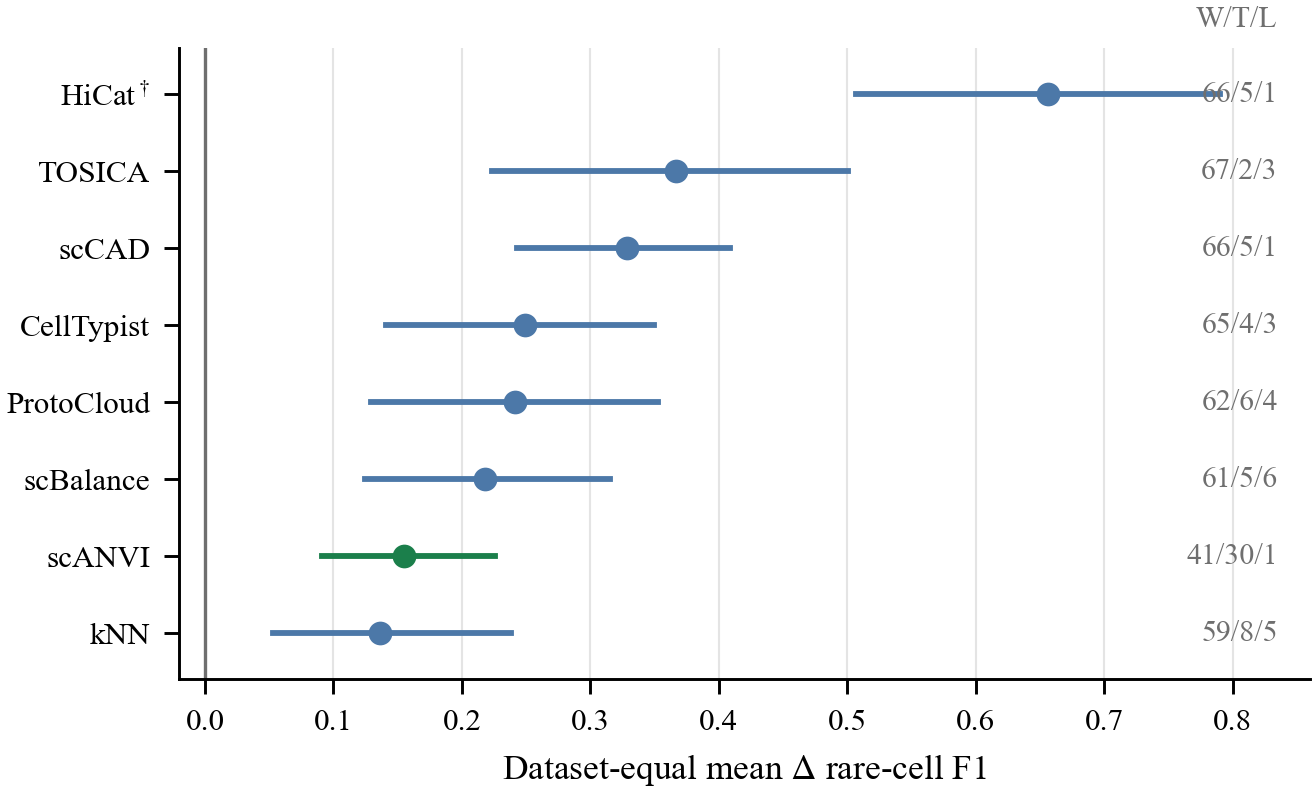
\includegraphics[width=0.72\linewidth]{fig4_paired_delta_forest.png}
\caption{稀缺标签区域的配对稀有 F1 增益。点表示\method 减去各比较方法所得的按数据集等权平均 $\Delta$F1，水平区间为通过数据集聚类重采样获得的 95\% 置信区间。右侧胜、平、负计数为匹配的数据集、预算和随机种子运行的描述性汇总。HiCat$^\dagger$ 为转导式参考。}
\label{fig:paired-delta}
\end{figure}

独立推断单位为数据集（$n=8$），因此置信区间仍对基准组成敏感。相对于 scANVI，逐一留出数据集后的平均效应范围为 $+0.1276$ 至 $+0.1766$，方向均未改变。将具有相同有效稀有标签数的名义预算合并后，敏感性分析得到相近的平均效应 $+0.1512$，95\% CI 为 $[+0.0885,+0.2232]$。这些分析不表示底层有标签细胞子集完全相同，结果表仅保留四位小数也限制了对极小差异的解释。

\subsection{观测总体稀有类假调用率经验上未超过参考预算}

只有在稀有标签保持特异性时，恢复更多稀有细胞才具有实际意义。在包含 \texttt{all} 标签预算的完整 8 数据集比较中，\method 观测到的最大总体稀有假调用率为 0.009878，低于预先指定的 $\alpha=0.01$ 预算。该最大值出现在 \texttt{mouse\_lung\_tms\_10x} 的一个随机种子、\rts{} $=$ \texttt{all} 设置中。在稀缺标签区域，最大值也接近但未超过同一预算。

各比较方法呈现不同安全性特征。kNN 和 scANVI 等方法假调用率较低，但会漏检较多稀有细胞。scCAD 等方法在本基准中恢复更多稀有细胞，但可能超过假调用预算。\method 位于预期的折中区域，在提高 scANVI 稀有召回率的同时，利用验证集校准抑制稀有标签的广泛扩张。该结论仅描述所评估运行中的经验约束，不构成对任意分布或完整选择流程的无条件 conformal 保证。

\subsection{跨组织与小鼠附加数据集支持更广泛的适用性证据}

原始人类基准涵盖免疫、胰腺、肺、胃和小肠。两个小鼠 Tabula Muris Senis 10x 附加数据集在保持相同评估约定的情况下，将覆盖扩展至第二个物种和额外组织。这些小鼠数据并非训练于人类细胞并测试于小鼠细胞的独立领域迁移实验，而是用于检验相同标签匮乏与拯救流程在原人类面板之外是否仍有用。纳入小鼠肺和小鼠胰腺降低了方法仅适配单一物种或组织几何结构的风险。主要聚合结果包含这两个数据集，完整结果表包含 864 个成功的方法级评估记录；这些记录覆盖不同方法，但不被视为相互独立的生物学重复。

\section{讨论}

核心结果表明，受约束的事后拯救模块能够恢复半监督骨干模型在严重标签匮乏条件下丢失的稀有细胞注释。\method 在 8 数据集基准中提高稀有细胞 F1 和召回率，；在所评估运行中，最终预测的观测总体稀有类假调用率经验上保持在 1\% 参考预算以内。方法的适用范围被有意限定为一个配置的低频目标类别。其原型仅由有标签训练细胞构建，阈值仅由验证细胞校准，并在验证证据不足时弃权。

这种限定具有实际价值。许多单细胞研究并不需要全新的注释模型，而需要判断一个小型已知细胞类型是否因类别不平衡与批次偏移而被抹去。由于\method 在 scANVI 之后运行，它可附加于既有半监督工作流，并通过门控、候选秩和校准阈值接受审计。当预测发生变化时，可追溯到潜在原型接近性与验证集校准的稀有分数证据；当预测不变时，弃权本身也提供信息。

评估还说明，稀有细胞基准应同时报告目标丰度和有标签稀有细胞可用性。低于 5\% 的目标类别在生物学上属于低频类别，但模型难度取决于训练集中保留多少有标签稀有样本。报告 $\lambda_\rare$ 可明确方法是在真实稀有标签区域中接受检验，而非仅在含低频类别的数据集上评估。

本研究存在若干限制。首先，\method 假设目标稀有类别预先已知，因此它是从头稀有细胞发现方法的补充，而非替代。其次，当前实现每次运行只细化一个目标稀有类别，多稀有类别设置可能需要逐类校准或联合误差预算分配。第三，方法继承 scANVI 潜在表示的质量。若稀有与多数细胞在潜在空间中不可分，保守门控将弃权，或召回率仍然受限。第四，虽然基准已加入小鼠数据，但尚未检验直接的人到小鼠模型迁移。最后，本文仅报告公共单细胞 RNA 测序数据的计算结果，对新恢复稀有细胞的实验验证仍需独立生物学测定或标志基因层面的确认。

\section{结论}

\method 为单细胞 RNA 测序注释中的已知低频细胞类型提供一种验证集校准的事后拯救流程。该方法结合仅由训练集得到的潜在原型、由验证集选择的候选秩、conformal 分数阈值及弃权门控，在严重稀有标签匮乏条件下提高稀有细胞恢复，并在所评估基准中对稀有假调用形成经验约束。当前 8 数据集基准支持将\method 作为一种实用细化模块，用于保留已知稀有细胞类型比最大化总体注释准确率更重要的研究场景。

\backmatter

\section*{数据可用性}

本研究所有数据均来自公开单细胞资源，包括人类图谱数据集以及 CELLxGENE/Tabula Muris Senis 小鼠 10x 子集。处理后数据集标识符、下载说明和预处理脚本将在代码仓库及补充数据中提供。本研究未生成新的测序数据。

\section*{代码可用性}

\method 实现、配置文件、比较脚本、绘图脚本和结果清单位于 \url{https://github.com/RanieZhou/scRareRefine.git}，许可证为 [license]。投稿版本将在 [Zenodo DOI] 归档。复现说明将包括比较网格使用的两个 conda 环境：用于 scANVI/\method 流程及多数基线的 \texttt{scanvi311}，以及用于需要旧版依赖栈基线的 \texttt{sandbox310}。

\section*{经费支持}

本研究由 [funding information] 支持。

\section*{利益冲突}

作者声明不存在利益冲突。

\section*{致谢}

作者感谢 scvi-tools、Scanpy、AnnData、CELLxGENE、Tabula Sapiens 和 Tabula Muris Senis 的维护者提供公开数据与软件资源。

\bibliography{sn-bibliography}

\end{document}